% !TEX encoding = UTF-8 Unicode.

% Based on https://github.com/Miracle0565/BUCT-Beamer-Theme

\documentclass[
10pt,
aspectratio=43,
]{beamer}
\setbeamercovered{transparent=10}
\usetheme[
%  showheader,
%  red,
  purple,
%  gray,
%  graytitle,
  colorblocks,
%  noframetitlerule,
]{Verona}

\usepackage[T1]{fontenc}
\usepackage{tikz}
\usepackage[utf8]{inputenc}
\usepackage{lipsum}
%%%%%%%%%%%%%%%%%%%%%%%%%%%%%%%
% Mac上使用如下命令声明隶书字体, windows也有相关方式, 大家可自行修改
\providecommand{\lishu}{\CJKfamily{zhli}}
%%%%%%%%%%%%%%%%%%%%%%%%%%%%%%%
\usepackage{tikz}
\usetikzlibrary{fadings}
%
%\setbeamertemplate{sections/subsections in toc}[ball]
\usepackage{xeCJK}
\usepackage{listings}
\usepackage{caption}
\usepackage{subfigure}
\usefonttheme{professionalfonts}
\def\mathfamilydefault{\rmdefault}
\usepackage{amsmath}
\usepackage{multirow}
\usepackage{booktabs}
\usepackage{bm}
\setbeamertemplate{section in toc}{\hspace*{1em}\inserttocsectionnumber.~\inserttocsection\par}
\setbeamertemplate{subsection in toc}{\hspace*{2em}\inserttocsectionnumber.\inserttocsubsectionnumber.~\inserttocsubsection\par}
\setbeamerfont{subsection in toc}{size=\small}
\AtBeginSection[]{%
	\begin{frame}%
		\frametitle{Outline}%
		\textbf{\tableofcontents[currentsection]} %
	\end{frame}%
}

\AtBeginSubsection[]{%
	\begin{frame}%
		\frametitle{Outline}%
		\textbf{\tableofcontents[currentsection, currentsubsection]} %
	\end{frame}%
}

\title{高等数学C}
%\subtitle{A Simple while elegant template}
\author[P.Yu]{余沛}
\mail{peiy\_gzgs@qq.com}
\institute[Guangzhou College of Technology and Business]{Guangzhou College of Technology and Business \\
  广州工商学院}
\date{\today}
\titlegraphic[width=4cm]{logo.png}{}




%%%%%%%%%%%%%%%%%%%%%%%%%%%%%%%%
% ----------- 标题页 ------------
%%%%%%%%%%%%%%%%%%%%%%%%%%%%%%%%



\begin{document}

\maketitle

%%% define code
\defverbatim[colored]\lstI{
	\begin{lstlisting}[language=C++,basicstyle=\ttfamily,keywordstyle=\color{red}]
	int main() {
	// Define variables at the beginning
	// of the block, as in C:
	CStash intStash, stringStash;
	int i;
	char* cp;
	ifstream in;
	string line;
	[...]
	\end{lstlisting}
}
%%%%%%%%%%%%%%%%%%%%%%%%%%%%%%%%
% ----------- FRAME ------------
%%%%%%%%%%%%%%%%%%%%%%%%%%%%%%%%

\section{变量变化问题}
\subsection{速度问题-I} % 匀速运动的情形
\begin{frame}{变量变化问题}{速度问题-I: 匀速运动的情形}
	考虑某物体 $A$ 以速度 $v$ 运动的情形, 记 $t$ 为物体运动的经过时间长度, $s$ 为物体在 $t$ 时刻运动的路程, 我们有
	\[
		s(t) = v\cdot t.
	\]

	\pause

	对于时刻 $t_1$, $t_2$ 来说, 我们有
	\[
		s(t_2) = v\cdot t_2 = v\cdot t_1 + v\cdot (t_2-t_1) = s(t_1) + v \cdot (t_2-t_1).
	\]
	\pause
	也就是说
	\[
		s(t_2) - s(t_1) = v \cdot (t_2-t_1), \quad v=\frac{s(t_2)-s(t_1)}{t_2-t_1}.
	\]
\end{frame}

\subsection{速度问题-II} % 匀加速运动的情形
\begin{frame}{变量变化问题}{速度问题-II: 匀加速运动的情形}
	考虑某物体 $A$ 以初速度 $v_0$, 加速度 $a$ 运动的情形, 记 $t$ 为物体运动的经过时间长度, $v(t)$ 为物体在$t$时刻的速度, $s(t)$ 为物体在 $t$ 时刻运动的路程, 我们有
	\[
		v(t) = v_0+a\cdot t.
	\]
	\pause
	对于时刻 $t_1$, $t_2$ 来说, 我们有
	\[
		v(t_2) = a\cdot t_2 = a\cdot t_1 + a\cdot (t_2-t_1) = v(t_1) + a \cdot (t_2-t_1).
	\]
	\pause
	也就是说
	\[
		v(t_2) - v(t_1) = a \cdot (t_2-t_1), \quad a=\frac{v(t_2)-v(t_1)}{t_2-t_1}.
	\]
\end{frame}

\begin{frame}{变量变化问题}{速度问题-II: 匀加速运动的情形}
	在前序知识中, 我们知道下式子以及相关的变形,
	\[
		s(t) = v_0\cdot t+ \frac{1}{2}a\cdot t^2
	\]
	\pause
	那么有
	\begin{align*}
		s(t_2) - s(t_1) & = v_0\cdot (t_2-t_1)+ \frac{1}{2}a\cdot (t_2^2-t_1^2)            \\
		                & =v_0\cdot(t_2-t_1) + a\cdot(t_2-t_1) \cdot \frac{1}{2}(t_2+t_1),
	\end{align*}
	\pause
	即
	\begin{align*}
		\frac{s(t_2) - s(t_1)}{t_2-t_1} = v_0 + a\cdot \frac{1}{2}(t_2+t_1).
	\end{align*}
	\pause
	对比匀速运动的速度定义, 我们可以看到, $t_1\sim t_2$ 期间的平均速度
	\begin{equation*}
		\tilde{v}=\frac{s(t_2) - s(t_1)}{t_2-t_1} = v_0 + a\cdot \frac{1}{2}(t_2+t_1).
	\end{equation*}
	\pause
	我们考虑速度 $t_2$, $t_1$ 足够接近的情况, $\lim_{(t_2-t_1)\to 0}\tilde{v}=v_0+a\cdot t_1$, 一致?
\end{frame}

\subsection{为什么要研究加速度的问题}
% 一般加速运动的情形
\begin{frame}
	\title{为什么要研究加速度的问题}
	\pause
	\begin{columns}
		\column{0.5\textwidth}
		\includegraphics<1->[width=\textwidth]{cat_guangzhou.jpg}

		\column{0.5\textwidth}
		\includegraphics<2->[width=\textwidth]{cat_gaza.jpg}
	\end{columns}

	\vspace{1cm}

	\begin{columns}
		\column{0.5\textwidth}
		\includegraphics<3->[width=\textwidth]{df17.jpg}

		\column{0.5\textwidth}
		\includegraphics<4->[width=\textwidth]{rajum.jpg}
	\end{columns}
\end{frame}

\begin{frame}
	\title{为什么要研究加速度的问题}
	\begin{columns}
		\column{0.5\textwidth}
		
\includegraphics[width=\textwidth]{cat_guangzhou.jpg}

		\column{0.5\textwidth}
		
\includegraphics[width=\textwidth]{cat_gaza.jpg}
	\end{columns}

	\vspace{1cm}

	\begin{columns}
		\column{0.5\textwidth}
		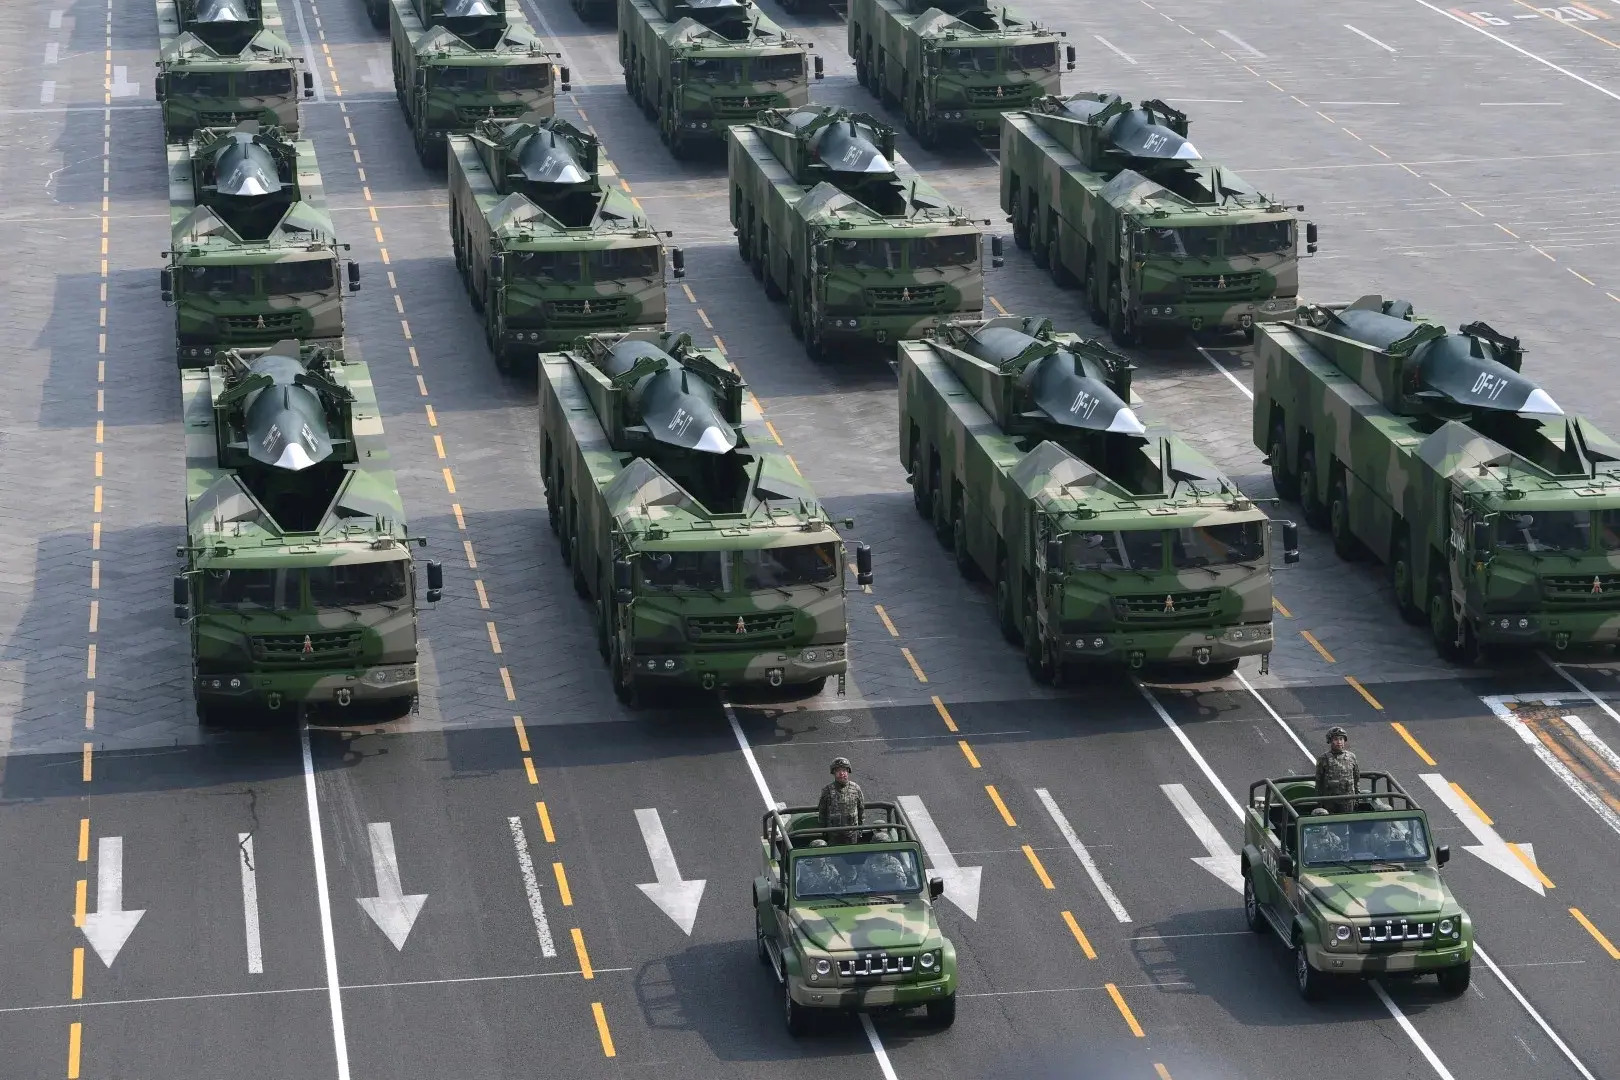
\includegraphics[width=\textwidth]{df17.jpg}

		\column{0.5\textwidth}
		
\includegraphics[width=\textwidth]{sling.jpeg}
	\end{columns}

\end{frame}


\subsection{速度问题-III}
\begin{frame}{变量变化问题}{速度问题-III: 一般运动的情形}
	\begin{exampleblock}{高超声速飞行器速度问题 \color{blue}(\small{\it 郭建国等, {现代防御技术}, 49(6) 2021.12.)}}
		平飞高超声速飞行器的加速度 $a$ 的简化计算模型为:
		\begin{align*}
			m\cdot a(t)= \frac{1}{2}\rho(s) v(t)^2 S C_T(t) - \frac{1}{2}\rho(s) v(t)^2 S C_D(s),
		\end{align*}
		其中, $m$ 是飞行器质量, $v(t)$ 是飞行器速度, $\rho(s)$ 是大气密度, $S$ 是飞行器截面积参考参数, $C_T$ 是油门控制值函数, $C_D$ 是该处的气动阻尼系数. 这种问题, 只给出$\rho(s)$, $S$, $C_T$ 和初速度, 如何计算路程和速度?
	\end{exampleblock}
	思路: 极限求 $v(t)$, 逐步求解. 对于 $t_2$, $t_1$ 足够接近的时候,
	\[
		v(t_2)\approx v(t_1)+a\left(\frac{t_2+t_1}{2}\right)(t_2-t_1).
	\]
	即
	\[
		\frac{v(t_2)-v(t_1)}{t_2-t_1}\approx a\left(\frac{t_2+t_1}{2}\right).
	\]
	因而, 我们会考虑相关的极限问题.
\end{frame}

\begin{frame}
	\frametitle{数学模型(第一页)}
	高超声速飞行器的纵向动力学模型如下:
	\[
		\begin{aligned}
			 & \dot{v}=\frac{T \cos \alpha-D}{m}-\frac{\mu \sin \gamma}{r^2}+w_1,                             \\
			 & \dot{h}=v \sin \gamma+w_2,                                                                     \\
			 & \dot{\gamma}=\frac{L+T \sin \alpha}{m v}-\frac{\left(\mu-v^2 r\right) \cos \gamma}{v r^2}+w_3, \\
			 & \dot{\alpha}=q-\dot{\gamma}+w_4,                                                               \\
			 & \dot{q}=\frac{M_{y y}}{I_{y y}}+w_5,
		\end{aligned}
	\]

	式中: $v$ 为飞行器速度; $h$ 为飞行器飞行高度; $\gamma$ 为飞行器航迹角; $\alpha$ 为飞行器攻角; $q$ 为俯仰角速度; $m$为飞行器质量; $I_{y y}$ 为转动惯量; 并且 $\mu$ 为重力常数; $w_i(i=1,2, \cdots, 5)$ 为不确定项.

\end{frame}

\begin{frame}
	\frametitle{数学模型(第二页)}

	气动力和力矩的表达式如下所示:

	\[
		\begin{aligned}
			 & T=\frac{1}{2} \rho v^2 S C_T, D=\frac{1}{2} \rho v^2 S C_D, L=\frac{1}{2} \rho v^2 S C_L,            \\
			 & M_{y y}=\frac{1}{2} \rho v^2 S c\left[C_M(\alpha)+C_M\left(\delta_{\mathrm{e}}\right)+C_M(q)\right], \\
			 & r=h+R_{\mathrm{E}},                                                                                  \\
			 & C_L=0.6203 \alpha, C_D=0.6450 \alpha^2+0.0043378 \alpha+0.003772,                                    \\
			 & C_T=\begin{cases}
				       0.02576 \beta,        & \text{if } \beta \leq 1, \\
				       0.0224+0.00336 \beta, & \text{otherwise},
			       \end{cases}                                                 \\
			 & C_M(\alpha)=-0.035 \alpha^2+0.036617(1+\Delta C_{M a}) \alpha+5.3261 \times 10^{-6},                 \\
			 & C_M(q)=\frac{\bar{c}}{2 v} q(-6.796 \alpha^2+0.3015 \alpha-0.2289),                                  \\
			 & C_M(\delta_{\mathrm{e}})=c_{\mathrm{e}}(\delta_{\mathrm{e}}-\alpha),
		\end{aligned}
	\]

	式中: $C_L$ 为升力系数; $C_D$ 为阻力系数; $C_T$ 为推力系数; $C_M(\cdot)$ 为力矩系数; $\rho, S, \bar{c}$ 以及 $R_{\mathrm{E}}$ 分别为大气密度、参考面积、平均空气动力弦和地球的半径.
\end{frame}
\begin{frame}
	\frametitle{数学模型(第三页)}

	发动机动力学模型如下

	\[
		\ddot{\beta}=-2 \xi \omega_{\mathrm{n}} \dot{\beta}-\omega_{\mathrm{n}}^2 \beta+\omega_{\mathrm{n}}^2 \beta_{\mathrm{c}},
	\]

	式中: $\beta, \beta_{\mathrm{c}}$ 分别为油门开度及油门开度指令; $\xi$ 为阻尼系数; $\omega_{\mathrm{n}}>0$ 为自然频率.
	
	\begin{figure}
		\centering
		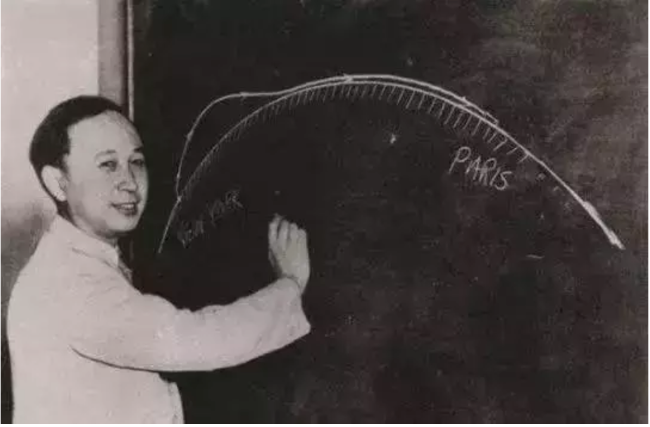
\includegraphics[width=0.5\textwidth]{qianxuesen.png}
		\caption{钱学森}
	\end{figure}

\end{frame}

\subsection{函数的切线问题-I} % 二次函数的切线问题

\begin{frame}{变量变化问题}{切线问题-I: 二次函数的情形}
	考虑二次函数
	\[
		f(x) = a\cdot x^2 + b\cdot x +c.
	\]
	\pause
	前序教育中, 给出了一些特殊函数的求导方法,
	\[
		k = f'(x_0) = 2  a \cdot x_0 + b
	\]
	\pause
	也定义了在某点上的切线方程,
	\[
		y = k \cdot x + (f(x_0) - k \cdot x_0),
	\]
	可以看到切线和导数之间具有某种关系.
\end{frame}

\subsection{函数的切线问题-II}
\begin{frame}{变量变化问题}{切线问题-II: 一般函数的情形}
    考虑函数 $f(x)$ 在点 $(x_0,f(x_0))$ 的切线问题.
    
    \pause
    考虑 $x_1<x_0<x_2$, 两点 $(x_1,f(x_1))$, $(x_2,f(x_2))$ 两点的割线斜率是
    \begin{equation*}
        k=\frac{f(x_2)-f(x_1)}{x_2-x_1},
    \end{equation*}
    \pause
    相关的割线方程是
    \begin{equation*}
        y-f(x_1)=k\cdot(x-x_1).
    \end{equation*}
    \pause
    \begin{center}
        
\includegraphics[scale=0.5]{tangent_secant_blank.png}
    \end{center}
    同样,用割线逼近切线, $x_1,x_2\to x_0$, $f(x)$ 的割线会慢慢逼近于切线
\end{frame}


\begin{frame}{变量变化问题}{切线问题-II: 一般函数的情形}
    考虑函数 $f(x)$ 在点 $(x_0,f(x_0))$ 的切线问题.

    考虑 $x_1<x_0<x_2$, 两点 $(x_1,f(x_1))$, $(x_2,f(x_2))$ 两点的割线斜率是
    \begin{equation*}
        k=\frac{f(x_2)-f(x_1)}{x_2-x_1},
    \end{equation*}
    相关的割线方程是
    \begin{equation*}
        y-f(x_1)=k\cdot(x-x_1).
    \end{equation*}
    \begin{center}
        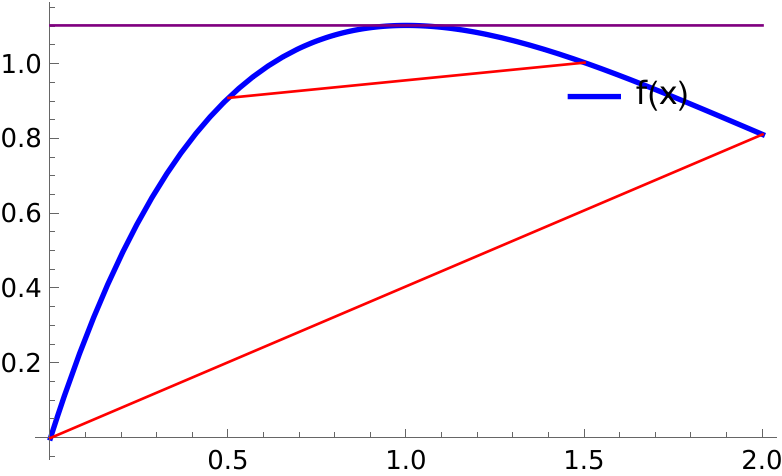
\includegraphics[scale=0.5]{tangent_secant.png}
    \end{center}
    同样,用割线逼近切线, $x_1,x_2\to x_0$, $f(x)$ 的割线会慢慢逼近于切线
\end{frame}




\section{导数}
\subsection{导数的定义}
\begin{frame}{导数的定义}
	\begin{block}{定义:函数导数}
		设 $f$, $\delta>0$ $(x_0-\delta,x_0+\delta)$, (或 $(x_0-\delta,x_0], [x_0,x_0+\delta)$) 上有定义, 对于 $0<\Delta x<\delta$, 如果极限
		\begin{equation*}
			\begin{array}[c]{c}
				\displaystyle\lim_{\Delta x\to 0 } \frac{f(x_0+\Delta x)-f(x_0)}{\Delta x},\bigskip \\
				\displaystyle\left(\text{或}\,\,\lim_{\Delta x\to0}\frac{f(x)-f(x-\Delta x)}{\Delta x}, \,\, \lim_{\Delta x\to0}\frac{f(x+\Delta x)-f(x)}{\Delta x} \right)
			\end{array}
		\end{equation*}
		存在, 则称 $f$ 在 $x_0$ 处{\bf 可导} (或{\bf 左导数存在}, {\bf 右导数存在}), 则称该极限值为 $f$ 在 $x_0$ 处的{\bf 导数} (或 左导数, 右导数), 记为 $f'(x_0)$ (或 $f'_-(x_0)$, $f'_+(x_0)$).
	\end{block}
	\pause
	若左右导数都存在且相等, 那么导数存在, 并与前两者的值相等.
\end{frame}

\begin{frame}{求导流程与微分概念}
	\begin{block}{求导流程: 差分 $\Delta y$, $\Delta x$ 的比较}
		\begin{enumerate}
			\pause\item 	给出 $\Delta x$; 算出 $\Delta y$; 求增量,
			      \pause\item  	求增量比 $\frac{\Delta y}{\Delta x}$; 求差商,
			      \pause\item  	求极限.
		\end{enumerate}
	\end{block}
	\pause
	\begin{block}{微分概念: 差分运算的形式化表示}
		设函数 $y=f(x)$, 在 $x_0$ 的某个邻域内有定义, 自变量在 $x_0$ 处取得增量 $\Delta x$, 因变量在 $f(x_0)$ 处取得增量 $\Delta y=f\left(x_0+\Delta x\right)-f\left(x_0\right)$,
		$$
			\Delta y=A \Delta x+o(\Delta x),
		$$
		其中 $\mathrm{A}$ 与 $x_0$ 有关而与 $\Delta x$ 无关, $o(\Delta x)$ 是比 $\Delta x$ 高阶的无穷小量. 那么称函数 $y=f(x)$ 在点 $x_0$ {\bf 可微}, $A \Delta x$ 称为微分, 即 $\mathrm{d} y=A \Delta x$. 由于 $\mathrm{d} x = \Delta x$, 记为
		$$
			\mathrm{d}y = A \mathrm{d}x.
		$$
	\end{block}
\end{frame}

\begin{frame}{求导流程与微分概念}
	\begin{block}{微分概念: 差分运算的形式化表示}
		设函数 $y=f(x)$, 在 $x_0$ 的某个邻域内有定义, 自变量在 $x_0$ 处取得增量 $\Delta x$, 因变量在 $f(x_0)$ 处取得增量 $\Delta y=f\left(x_0+\Delta x\right)-f\left(x_0\right)$,
		$$
			\Delta y=A \Delta x+o(\Delta x),
		$$
		其中 $\mathrm{A}$ 与 $x_0$ 有关而与 $\Delta x$ 无关, $o(\Delta x)$ 是比 $\Delta x$ 高阶的无穷小量. 那么称函数 $y=f(x)$ 在点 $x_0$ {\bf 可微}, $A \Delta x$ 称为微分, 即 $\mathrm{d} y=A \Delta x$. 由于 $\mathrm{d} x = \Delta x$, 记为
		$$
			\mathrm{d}y = A \mathrm{d}x.
		$$
	\end{block}
	\pause
	请注意, 微分记号适用于进行"考虑差分$-$计算增量$-$对增量变化比例求极限"的过程. 因此, 微分运算的本质是一种"省略" 以加速对函数性质的理解和计算; 也是因此, 在理解和计算中出现疑惑时\dots
	\pause
	\begin{exampleblock}{}
		{\large ``请循其本.''}
		\hspace*\fill{\small--- 庄子, to 惠子, 《庄子与惠子游于濠梁之上》,	战国中期.}
	\end{exampleblock}
\end{frame}

\begin{frame}{导数与微分的关系}
	\begin{theorem}
		函数 $y=f(x)$ 在点 $x_0$ 处可微的定义的充分必要条件是函数 $y=f(x)$ 在点 $x_0$ 处可导.
	\end{theorem}{}
	\bigskip\bigskip\pause
	\begin{exampleblock}{}
		\begin{center}
			$\displaystyle\frac{\mathrm{d}y}{\mathrm{d}x}=f'(x),\qquad$可导 $\Longleftrightarrow$ 可微 $\Rightarrow$ 连续 $\Rightarrow$ 极限存在.
		\end{center}
	\end{exampleblock}

\end{frame}


\begin{frame}{一些导数计算例子}
	\begin{block}{例子}
		\begin{enumerate}
			\item $f(x)=C$, \pause $f'(x) =0$;\pause
			\item $f(x)=x^n, (n\in\mathbb{N}^+)$, \pause $f'(x) = n x^{n-1}$;\pause
			\item $f(x)=\sin(x)$, \pause $f'(x)=\cos(x)$; \,\,\pause $g(x)=\cos(x)$, \pause $g'(x)=-\sin(x)$;\pause
			\item $f(x)=\log_a  x$,\,\pause $f'(x)=\log a \cdot \displaystyle\frac{1}{x}$
		\end{enumerate}
	\end{block}
\end{frame}

\subsection{导数的四则运算法则}
\begin{frame}{函数和差的导数}
	\begin{block}{函数和差的导数}
		设 $f(x)$, $g(x)$ 在 $x_0$ 处有导数, 那么有
		\[
			(f(x_0)\pm g(x_0))' = f'(x_0)\pm g'(x_0).
		\]
	\end{block}
	\pause
	Why?
	\pause
	\begin{align*}
		  & \frac{(f(x_0+\Delta x)\pm g(x_0+\Delta x))-(f(x_0)\pm g(x_0))}{\Delta x}                  \\
		= & \frac{f(x_0+\Delta x)-f(x_0)}{\Delta x}\pm \frac{( g(x_0+\Delta x))-( g(x_0))}{\Delta x}.
	\end{align*}
\end{frame}

\begin{frame}{函数和差的导数}{导数计算题目}
	\begin{block}{题目}
		计算以下函数的导数:
		\begin{enumerate}
			\item $f(x) = 1 + x$,
			\item $g(x) = x + \sin(x)$,
			\item $h(x) = \cos(x) + \log(x)$,
		\end{enumerate}
	\end{block}

	\pause

	\begin{block}{答案}
		\begin{enumerate}
			\item $f'(x) = 1$,
			\item $g'(x) = 1 + \cos(x)$,
			\item $h'(x) = -\sin(x) + \displaystyle\frac{1}{x}$,
		\end{enumerate}
	\end{block}
\end{frame}

\begin{frame}{函数乘积的导数}
	\begin{block}{函数乘积的导数}
		设 $f(x)$, $g(x)$ 在 $x_0$ 处有导数, 那么有
		\[
			(f(x_0)\cdot g(x_0))' = f'(x_0)\cdot g(x_0) + f(x_0)\cdot g'(x_0).
		\]
	\end{block}
	\pause
	Why?
	\pause
	\begin{align*}
		  & f(x_0+\Delta x)g(x_0+\Delta x)-f(x_0) g(x_0))                                                 \\\bigskip
		= & \left(f(x_0+\Delta x)g(x_0+\Delta x)-f(x_0) g(x_0+\Delta x)\right)                            \\\smallskip
		  & + \left(f(x_0)g(x_0+\Delta x)-f(x_0) g(x_0)\right)                                            \\\bigskip
		= & \left(f(x_0+\Delta x)-f(x_0)\right)g(x_0+\Delta x)+f(x_0)\left(g(x_0+\Delta x)-g(x_0)\right).
	\end{align*}
\end{frame}

\begin{frame}
	\frametitle{函数乘积的导数}{导数计算题目}
	\begin{exampleblock}{题目}
		计算以下函数的导数:
		\begin{enumerate}
			\item $f(x) = x \log(x)$,
			\item $g(x) = x \sin(x)$,
			\item $h(x) = \sin(x) \cos(x) \log(x)$,
		\end{enumerate}
	\end{exampleblock}

	\pause

	\begin{exampleblock}{答案}
		\begin{enumerate}
			\item $f'(x) = \log(x) + 1$,
			\item $g'(x) = \sin(x) + x \cos(x)$,
			\item $h'(x) = \cos^2(x) \log(x) - \sin^2(x) \log(x) + \displaystyle\frac{\sin(x)\cos(x)}{x}$,
		\end{enumerate}
	\end{exampleblock}
\end{frame}

\begin{frame}{函数商的导数}
	\begin{block}{函数商的导数}
		设 $f(x)$, $g(x)$ 在 $x_0$ 处有导数, 且 $g'(x_0)\neq 0$, 那么有
		\[
			\left(\frac{f(x_0)}{g(x_0)}\right)' = \frac{f'(x_0)g(x_0)-g'(x_0)f(x_0)}{(g(x_0))^2}
		\]
	\end{block}
	Why?
	\begin{align*}
		  & \frac{f(x_0+\Delta x)}{g(x_0+\Delta x)}-\frac{f(x_0)}{g(x_0)}                                                \\\bigskip
		= & \frac{f(x_0+\Delta x)g(x_0)-f(x_0)g(x_0+\Delta x)}{g(x_0+\Delta x)g(x_0)}                                    \\\bigskip
		= & \frac{f(x_0+\Delta x)g(x_0)-f(x_0)g(x_0)+f(x_0)g(x_0)-f(x_0)g(x_0+\Delta x)}{g(x_0+\Delta x)g}               \\\bigskip
		= & \frac{\left(f(x_0+\Delta x)-f(x_0)\right)g(x_0)-f(x_0)\left(g(x_0+\Delta x)-g(x_0)\right)}{g(x_0+\Delta x)g}
	\end{align*}
\end{frame}

\begin{frame}{函数商的导数}
	\frametitle{函数商的导数}{导数计算题目}
	\begin{exampleblock}{题目}
		计算以下函数的导数:
		\begin{enumerate}
			\item $f(x) = \sec(x)$, 注: $\left(\sec(x)=\displaystyle\frac{1}{\cos(x)}\right),$
			\item $g(x) = \tan(x)$,
			\item $h(x) = \displaystyle\frac{\cos(x)}{\log(x)}$,
		\end{enumerate}
	\end{exampleblock}

	\pause

	\begin{exampleblock}{答案}
		\begin{enumerate}
			\item $f'(x) = \sec(x) \tan(x)$,
			\item $g'(x) = \sec^2(x)$,
			\item $h'(x) = \displaystyle\frac{-\sin(x)\log(x)-\displaystyle\frac{\cos(x)}{x}}{(\log(x))^2}$,
		\end{enumerate}
	\end{exampleblock}
\end{frame}

\begin{frame}{相关的微分计算法则}
	\begin{alertblock}{微分计算法则}
		假如函数 $u=u(x), v=v(x)$ 可微, 那么有
		\begin{itemize}
			\item $d(u \pm v) = du \pm dv$,
			\item $d(Cu) = C du$,
			\item $d(uv) = v du + u dv$,
			\item $\displaystyle d\left(\frac{u}{v}\right) = \frac{v du - u dv}{v^2}$, ($v \neq 0$).
		\end{itemize}
	\end{alertblock}
\end{frame}

\begin{frame}
	\frametitle{反函数求导定理}
	\begin{theorem}[反函数求导定理]
		若函数 $y=f(x)$ 在 $(a, b)$ 上连续、严格单调、可导并且 $f'(x) \neq 0$, 记 $\alpha=\min(f(a+), f(b-))$, $\beta=\max(f(a+), f(b-))$, 则它的反函数 $x=f^{-1}(y)$ 在 $(\alpha, \beta)$ 上可导, 且有
		\[
			\left[f^{-1}(y)\right]' = \frac{1}{f'(x)}.
		\]
	\end{theorem}
	\begin{exampleblock}{简单观察}
		\begin{equation*}
			y=f(x)\rightleftarrows\frac{\mathrm{d}y}{\mathrm{d}x}=f'(x).
		\end{equation*}
		and
		\begin{equation*}
			x=f^{-1}(y)\rightleftarrows\left[f^{-1}(y)\right]'=\frac{\mathrm{d}x}{\mathrm{d}y}=\left(\frac{\mathrm{d}y}{\mathrm{d}x}\right)^{-1}=(f'(x))^{-1}.
		\end{equation*}

	\end{exampleblock}
\end{frame}

\begin{frame}
	\frametitle{反函数求导定理}
	\begin{proof}
		因为函数 $y=f(x)$ 在 $(a, b)$ 上连续且严格单调, 由反函数连续定理, 它的反函数 $x=f^{-1}(y)$ 在 $(\alpha, \beta)$ 上存在、连续, 且严格单调. 这时 $\Delta y=f(x+\Delta x)-f(x) \neq 0$ 等价于 $\Delta x=f^{-1}(y+\Delta y)-f^{-1}(y) \neq 0$, 并且当 $\Delta y \rightarrow 0$ 时有 $\Delta x \rightarrow 0$.因此
		\[
			\begin{aligned}
				\left[f^{-1}(y)\right]' & = \lim_{\Delta y \rightarrow 0} \frac{f^{-1}(y+\Delta y)-f^{-1}(y)}{\Delta y} \\
				                        & = \lim_{\Delta x \rightarrow 0} \frac{\Delta x}{f(x+\Delta x)-f(x)}           \\
				                        & = \frac{1}{\lim_{\Delta x \rightarrow 0} \frac{f(x+\Delta x)-f(x)}{\Delta x}} \\
				                        & = \frac{1}{f'(x)}.
			\end{aligned}
		\]
	\end{proof}
\end{frame}

\begin{frame}
	\frametitle{导数计算题目}
	\begin{exampleblock}{题目}
		计算以下函数的导数:
		\begin{enumerate}
			\item $f(x) = e^x,$
			\item $g(x) = \arcsin(x),$
			\item $h(x) = \arccos(x).$
		\end{enumerate}
	\end{exampleblock}

	\pause

	\begin{exampleblock}{答案}
		\begin{enumerate}
			\item $f'(x) = e^x$, 令 $y=e^x$, 有 $x=\log y$ 和 $(e^x)'=\displaystyle\frac{1}{(\log y)'}=y=e^x,$
			\item $g'(x) = \displaystyle\frac{1}{\sqrt{1-x^2}},$ $(\arcsin(x))'=\displaystyle\frac{1}{(\sin (y))'}=\frac{1}{\cos(y)}=\frac{1}{\sqrt{1-(\sin(y))^2}}=\frac{1}{\sqrt{1-x^2}},$
			\item $h'(x) = -\displaystyle\frac{1}{\sqrt{1-x^2}},$ 类似的, $(\arcsin(x))'=\displaystyle\frac{1}{(\sin (y))'}=-\frac{1}{\sqrt{1-x^2}}.$
		\end{enumerate}
	\end{exampleblock}
\end{frame}


\subsection{复合函数的求导法则}
\begin{frame}{复合函数的求导法则}
	\begin{block}{链式求导法则}
		如果 $u=\varphi(x)$ 在 $x=x_0$ 点可导, 且 $y=f(u)$, $u=u_0=\varphi\left(x_0\right)$ 点也可导, 那么, 复合函数 $f(\varphi(x))$ 在 $x=x_0$ 点可导
		\[
			[f(\varphi(x))]_{x=x_0}^{\prime}=f^{\prime}\left(u_0\right) \varphi^{\prime}\left(x_0\right),
		\]
		以及
		\[
			\mathrm{d}y=f'(u)du=f'(u)\varphi'(x)\mathrm{d}x.
		\]
	\end{block}
	Why? \pause 考虑 $\Delta u = u(x_0+\Delta x) - u(x_0)$, \pause 由连续性, 有$\lim_{\Delta x\to0}\Delta u=0$ \pause
	\begin{align*}
		f\left(u_0+\Delta u\right)-f\left(u_0\right)=f^{\prime}\left(u_0\right) \Delta u+\alpha(\Delta u) \Delta u
	\end{align*}
	其中 $\lim_{\Delta x\to0}\alpha(\Delta u)=0$. \pause Why? \pause
	\begin{align*}
		\lim _{\Delta x \rightarrow 0} \frac{f\left(g\left(x_0+\Delta x\right)\right)-f\left(g\left(x_0\right)\right)}{\Delta x}= & f^{\prime}\left(u_0\right) \lim _{\Delta x \rightarrow 0} \frac{\Delta u}{\Delta x}+\lim _{\Delta x \rightarrow 0} \alpha \lim _{\Delta x \rightarrow 0} \frac{\Delta u}{\Delta x} \\
		=                                                                                                                         & f^{\prime}\left(u_0\right)f^{\prime}\left(x_0\right).
	\end{align*}
\end{frame}


\begin{frame}
	\frametitle{导数计算题目}
	\begin{block}{幂指函数的导数计算}
		假设 $f$, $g$ 在所考虑的区域上可导, 如何形如以下的函数
		\[
			h(x)=f(x)^{g(x)}.
		\]
	\end{block}

	\pause

	\begin{exampleblock}{方法}
		在等式两边求对数, 有
		\[
			\log h(x) = g(x)\log (f(x)),
		\]
		因此, 有
		\begin{align*}
			\displaystyle\frac{h'(x)}{h(x)} & =(\log h(x))' = (g(x)\log (f(x)))'                                     \\
			h'(x)                           & =\displaystyle h(x)\left(g'(x)\log(f(x))+g(x)\frac{f'(x)}{f(x)}\right)
		\end{align*}
	\end{exampleblock}
\end{frame}

\subsection{隐函数求导法则}
\begin{frame}{隐函数求导法则}
	\begin{block}{隐函数求导法则}
		设函数 $F(x, y) = 0$ 定义了一个隐函数 $y = f(x)$, 其中 $F$ 是可微函数.则隐函数的导数可以通过以下公式计算:
		\[
			d F(x, y)=\partial_xF(x,y) d x+\partial_yF(x,y) d y=0,\,\,\,\, \frac{\mathrm{d}y}{\mathrm{d}x} = -\frac{\displaystyle\,\,{\frac{{\partial F}}{{\partial x}}}\,\,}{{\displaystyle\frac{{\partial F}}{{\partial y}}}}.
		\]
	\end{block}

	\pause

	\begin{example}
		考虑方程 $\mathrm{e}^{x+y}=xy$, 我们可以将其视为隐函数 $y = f(x)$.通过隐函数求导法则, 我们可以计算出导数为:
		\[
			\displaystyle\frac{{dy}}{{dx}} = -\displaystyle\frac{\,\,{\displaystyle\frac{{\partial (\mathrm{e}^{x+y}-xy)}}{{\partial x}}}\,\,}{{\displaystyle\frac{{\partial (\mathrm{e}^{x+y}-xy)}}{{\partial y}}}} = -\frac{{(\mathrm{e}^{x+y}-y)}}{{(\mathrm{e}^{x+y}-x)}}.
		\]
	\end{example}
\end{frame}

\begin{frame}{隐函数求导法则}
	\begin{block}{题目}
		\begin{itemize}
			\item 方程 $x^2 + y^2 = 1$ 定义了一个隐函数 $y = f(x)$.
			\item 方程 $\displaystyle\mathrm{e}^{x+y}=\frac{x}{y}$ 定义了一个隐函数 $y = g(x)$.
			\item 方程 $x^3 + y^3 = 9xy$ 定义了一个隐函数 $y = h(x)$.
		\end{itemize}
	\end{block}

	\pause

	\begin{exampleblock}{答案}
		\begin{itemize}
			\item 隐函数 $y = f(x)$ 的导数为 $\displaystyle\frac{{dy}}{{dx}} = -\frac{{x}}{{y}}.$
			\item 隐函数 $y = g(x)$ 的导数为 $\displaystyle\frac{{dy}}{{dx}} = -\frac{{\mathrm{e}^{x+y}-y}}{{\mathrm{e}^{x+y}-\frac{x}{y}}}.$
			\item 隐函数 $y = h(x)$ 的导数为 $\displaystyle\frac{{dy}}{{dx}} = -\frac{{3x^2 - 3y^2}}{{3y^2 - 3x^2}}.$
		\end{itemize}
	\end{exampleblock}
\end{frame}

\subsection{常见导数计算结果}
\begin{frame}{算例}
	\begin{block}{}
		{\small 基本结果:
			\begin{enumerate}
				\item $f(x)=C$,  $f'(x) =0$;
				\item $f(x)=x^n, (n\in\mathbb{N}^+)$,  $f'(x) = n x^{n-1}$;
				\item $f(x)=\sin(x)$,  $f'(x)=\cos(x)$; \,\, $g(x)=\cos(x)$,  $g'(x)=-\sin(x)$;
				\item $f(x)=\log_a  x$,\, $f'(x)= \displaystyle\frac{1}{\log a \cdot x}$;
			\end{enumerate}
			利用反函数和复合函数法则后:
			\begin{enumerate}
				\item $f(x) = e^x$, $f'(x) = e^x$; $f(x)=a^x(a>0)$, $f'(x)=\log a \cdot a^x$
				\item $f(x) = \arcsin(x)$, $f'(x) = \displaystyle\frac{1}{\sqrt{1-x^2}}$, $g(x) = \arccos(x)$, $g'(x) = \displaystyle-\frac{1}{\sqrt{1-x^2}}$;
				\item $f(x) = \arctan(x)$, $f'(x) = \displaystyle\frac{1}{1-x^2}$;
				\item $f(x) = x^a,\,\,(a\neq0)$, $\displaystyle\frac{f'(x)}{f(x)}=\left(\log(f(x))\right)'=a\cdot \frac 1x$, $\displaystyle f'(x)=a\cdot\frac1x\cdot f(x)=ax^{a-1}$.
			\end{enumerate}
		}
	\end{block}
\end{frame}



\subsection{高阶导数和高阶微分}
\begin{frame}
	\frametitle{递归定义高阶导数和高阶微分}

	\begin{block}{高阶导数和高阶微分:递归定义}
		设 $f(x)$ 是一个可导函数, 定义 $f^{(0)}(x) = f(x)$, 则对于任意正整数 $n$, 假如以下运算都可以进行, 可以递归地定义高阶导数和高阶微分为
		\[
			f^{(n)}(x) := \left(f^{(n-1)}(x)\right)',\,\,\frac{\mathrm{d}^n}{\mathrm{d}x^n}f=\frac{\mathrm{d}^nf}{\mathrm{d}x^n}:= \frac{\mathrm{d}\frac{\mathrm{d}^{n-1}}{\mathrm{d}x^{n-1}}f}{\mathrm{d}x}=\frac{\mathrm{d}}{\mathrm{d}x}\frac{\mathrm{d}^{n-1}}{\mathrm{d}x^{n-1}}.
		\]
	\end{block}
	\pause
	\begin{exampleblock}{高阶导数计算法则}
		设 $f(x)$ 和 $g(x)$ 是可导函数,$n$ 是正整数,$a$ 是常数,则有以下法则:

		\begin{itemize}
			\item 和差法则:$(f \pm g)^{(n)}(x) = f^{(n)}(x) \pm g^{(n)}(x)$,

			\item 数乘法则:$(af)^{(n)}(x) = a \cdot f^{(n)}(x)$,

			\item Liebniz 法则:$\displaystyle(f \cdot g)^{(n)}(x) = \sum_{k=0}^{n} C_n^k f^{(k)}(x) \cdot g^{(n-k)}(x)$.
		\end{itemize}
	\end{exampleblock}
	例题: $y=x^2 e^{2 x}$, 求 $y^{(3)}$. \pause
\end{frame}
\subsection{证明算例}

\begin{frame}
	\frametitle{证明$f(x)=x\sin\left(\frac{1}{x}\right)$在零点不可导}
	\begin{exampleblock}{习题}
		证明函数
		\[
			f(x) = \begin{cases}
				\displaystyle x\sin\left(\frac{1}{x}\right), & \text{if } x, \neq 0, \\
				0,                                           & \text{if } x = 0.
			\end{cases}
		\]
		在零点不可导.
	\end{exampleblock}
	这其实也是一个例子, 说明函数低阶可导并不能说明函数高阶可导.
\end{frame}

\begin{frame}
	\frametitle{证明$f(x)=x\sin\left(\frac{1}{x}\right)$在零点不可导}

	\begin{block}{proof.}
		当 $x\neq0$时, $f'(x)$ 有
		\[
			f'(x) = \left(x\right)' \sin\left(\frac{1}{x}\right) + x \left(\sin\left(\frac{1}{x}\right)\right)'
		\]
		接下来, 我们计算每一项的导数:
		\[
			\left(\sin\left(\frac{1}{x}\right)\right)' = \cos\left(\frac{1}{x}\right) \cdot \left(\frac{1}{x}\right)'
		\]
		由于$\left(\frac{1}{x}\right)' = -\frac{1}{x^2}$, 我们可以将上式简化为:
		\[
			\left(\sin\left(\frac{1}{x}\right)\right)' = \cos\left(\frac{1}{x}\right) \cdot \left(-\frac{1}{x^2}\right) = -\frac{\cos\left(\frac{1}{x}\right)}{x^2}
		\]
	\end{block}
\end{frame}

\begin{frame}
	\frametitle{证明$f(x)=x\sin\left(\frac{1}{x}\right)$在零点不可导}

	\begin{proof}
		当 $x\neq0$时, 将以上结果代入乘积法则的公式中, 我们得到
		\[
			f'(x) = 1 \cdot \sin\left(\frac{1}{x}\right) + x \cdot \left(-\frac{\cos\left(\frac{1}{x}\right)}{x^2}\right)
		\]
		选取左,右点列分别为:
		\[
			x_{k_1}=-\displaystyle\frac{1}{2k_1\pi+\frac{\pi}{2}},\,\,x_{k_2}=-\displaystyle\frac{1}{2k_2\pi+\frac{\pi}{2}}.
		\]
		可以看到左右导数在 $x=0$ 点不相等, 因此该函数在 $x=0$ 点不可导.
	\end{proof}
\end{frame}




\beamertemplateshadingbackground{structure.fg!90}{structure.fg}
\begin{frame}[plain]
	\vfill
	\centering
	{
		\centering \Huge \color{white} Thank you for your attention!\\[10pt]Questions?\\\bigskip
		Homework: Page 119: 1, 3, 10; Page 120: 17, 23, 26.
	}
	\vfill
\end{frame}


\end{document}
